\documentclass[a4paper,12pt]{article}

%%% Работа с русским языком
\usepackage{cmap}					% поиск в PDF
\usepackage{mathtext} 				% русские буквы в фомулах
\usepackage[T2A]{fontenc}			% кодировка
\usepackage[utf8]{inputenc}			% кодировка исходного текста
%\usepackage[english]{babel}	% локализация и переносы

%%% Дополнительная работа с математикой
\usepackage{amsfonts,amssymb,amsthm,mathtools} % AMS
\usepackage{amsmath}
\usepackage{icomma} % "Умная" запятая: $0,2$ --- число, $0, 2$ --- перечисление

%% Номера формул
%\mathtoolsset{showonlyrefs=true} % Показывать номера только у тех формул, на которые есть \eqref{} в тексте.

\usepackage{hyperref}
\hypersetup{
    colorlinks=false,
    linkcolor=blue,
    filecolor=magenta,      
    urlcolor=cyan,
}

\usepackage{float}
\usepackage{indentfirst}
\usepackage{pdfpages}


%% Шрифты
\usepackage{euscript}	 % Шрифт Евклид
\usepackage{mathrsfs} % Красивый матшрифт

%%% Работа с картинками
\usepackage{graphicx}  % Для вставки рисунков
\graphicspath{{images/}{images2/}}  % папки с картинками
\setlength\fboxsep{3pt} % Отступ рамки \fbox{} от рисунка
\setlength\fboxrule{1pt} % Толщина линий рамки \fbox{}
\usepackage{wrapfig} % Обтекание рисунков и таблиц текстом
\usepackage{caption}
\usepackage{subcaption}
\captionsetup{labelsep=period} %. вместо : в рис

\title{Properies of magnetic models on ensembles of conformations}
%\title{PROPERTIES OF MAGNETIC MODELS ON ENSEMBLES OF CONFORMATIONS}
\author{Moskalenko R. B.}

\begin{document}
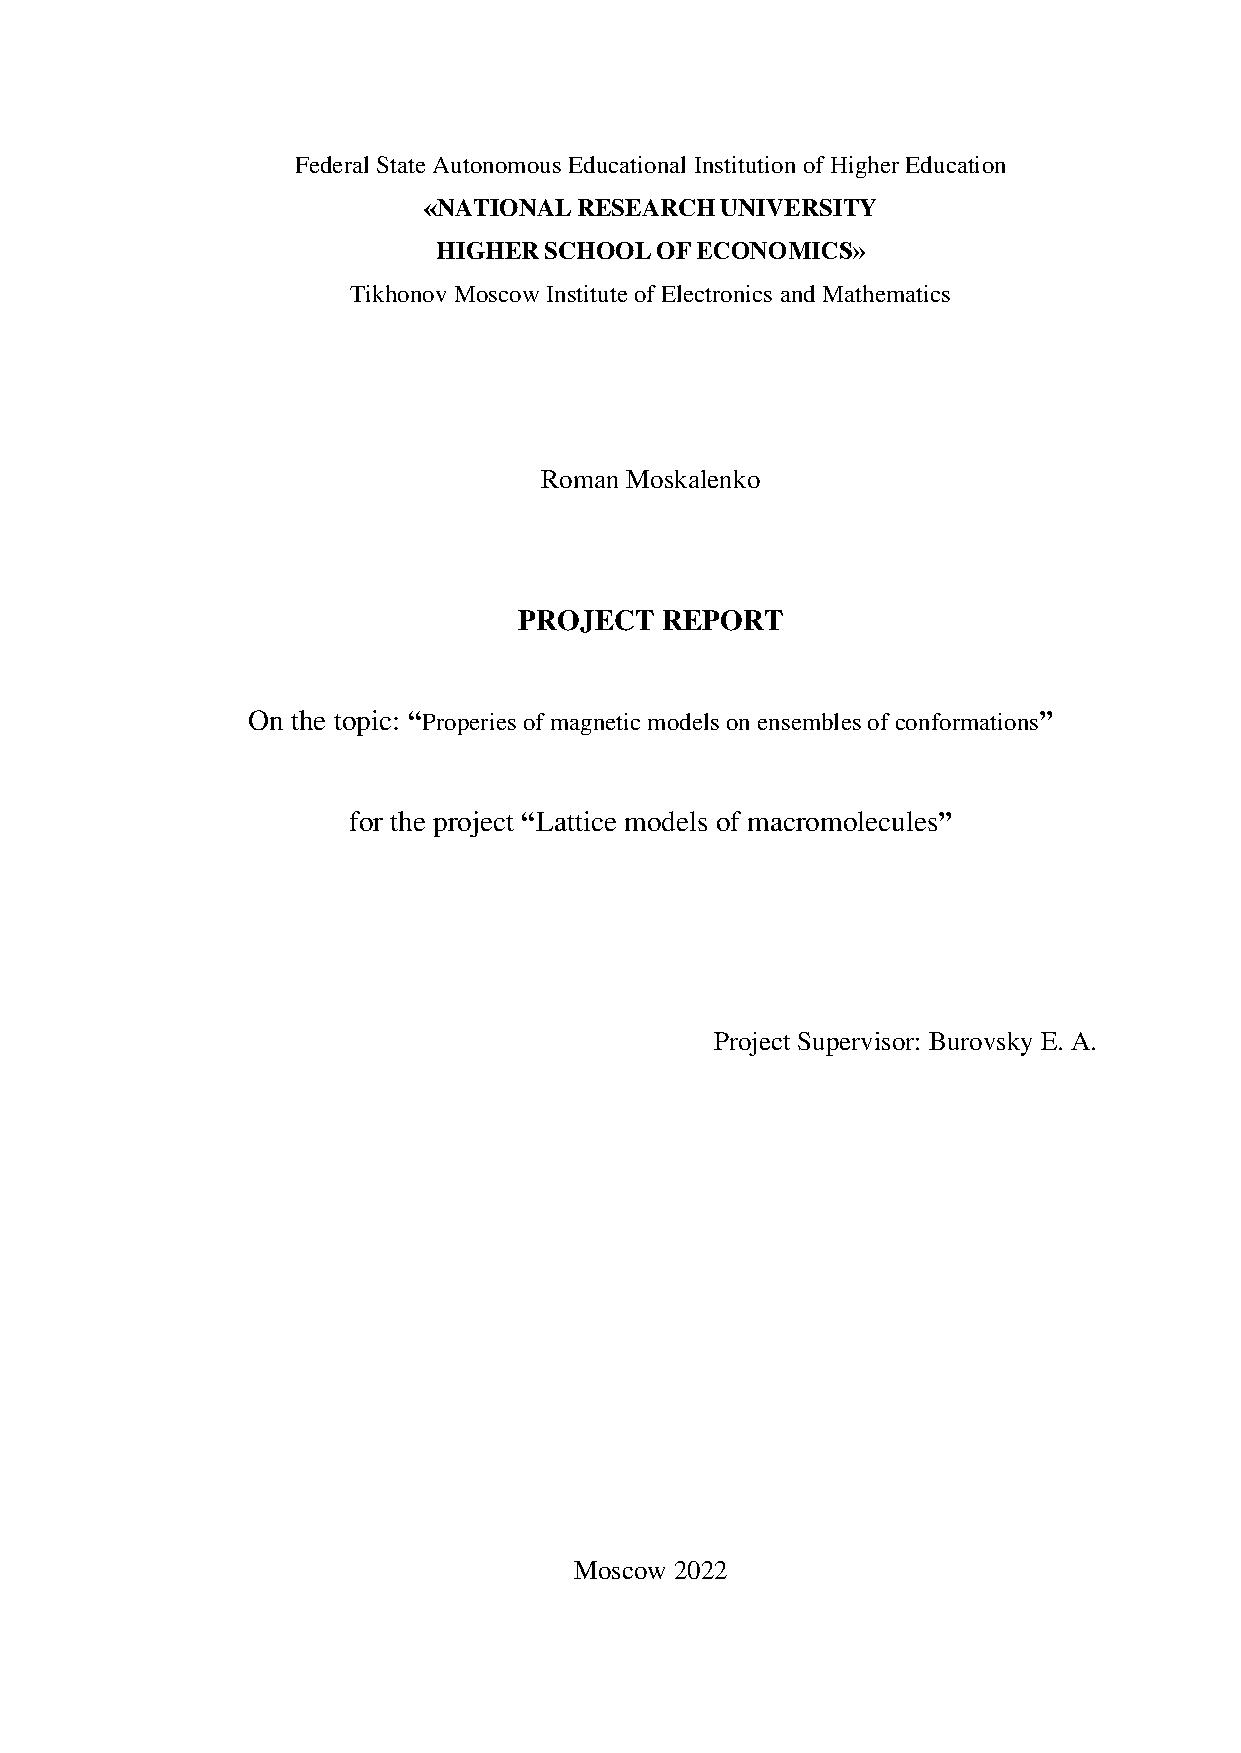
\includepdf[pages={1}]{Report_eng_title.pdf}

\section*{Summary}
In this project, we study magnetic properties of macromolecules by modeling it using Ising model on conformations. The goal of the project is to find magnetic transition point which should appear after geometric transition in globular state. It will show how geometric properties of macromolecules correlate with magnetic properties.

\section*{Project overview}
Representation of a macromolecule as a random walk on a regular lattice is a fairly new, but a well researched subject. These random walks called conformations, and resent studies has shown, that conformations has geometric transition. There are two states: coil and globule - which correspond to high and low temperatures. Ising model\cite{Ising_model} is another well researched model, which is used to calculate magnetic properties of grid-based structures. And it is known that two-dimensional grid has a magnetic transition, but one-dimensional grid does not.

If we look at the conformations (fig.\ref{fig:conf_example}) we can see that globule and coil conformations closely resemble one and two-dimensional grids respectively. We can assume that they have similar magnetic properties, and more specifically: globule conformations have magnetic transition and coil conformations don't. So, the goal of this project is to prove that globule conformations have a magnetic transition, find the transition point and compare it to the geometric transition point.

\begin{figure}[h]
	\centering
	\begin{subfigure}[t]{0.3\textwidth}
		\centering
		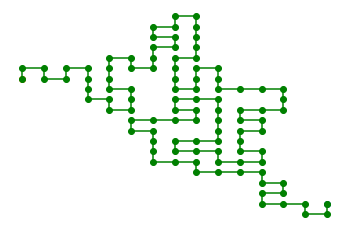
\includegraphics[width=\textwidth]{images/dense_conf.png} 
		\caption{Globule}
	\end{subfigure}
	\begin{subfigure}[t]{0.3\textwidth}
		\centering
		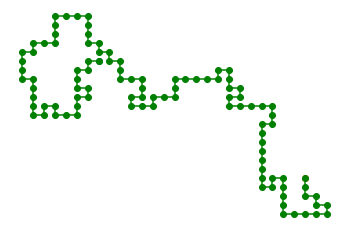
\includegraphics[width=\textwidth]{images/loose_conf.png} 
		\caption{Coil}
	\end{subfigure}
	\caption{Example of globule and coil conformations}
	\label{fig:conf_example}
\end{figure}

\section*{Proposed solution}
To collect data, we use computer simulations. Firstly, we generate a set of conformations using the SAW algorithm. All conformations are generated with the same length and at the same temperature. On each of the conformations, we simulate Ising model with different temperatures(not the same temperature as in SAW). We simulate Ising model using Wolff's algorithm\cite{wolff_algo} with cluster update, which is a Monte Carlo method that allows us to statistically determine magnetic properties of Ising model without calculation of all possible spin configurations. All calculations are done on the supercomputer cluster of HSE\cite{supercomputer}, code can be found on GitHub\cite{github}.

After simulation is completed, we calculate Binder cumulant\cite{Binder_cumulant}, using formula \ref{cumulant_eq}, for all conformations with the same length.
\begin{equation}
	U = 1 - \frac{\langle m^4\rangle}{3\langle m^2\rangle ^ 2}
	\label{cumulant_eq}
\end{equation}
Then, if we calculate mean cumulant for different lengths of conformations and plot them, we should see that that all graphs intersect at one point. The point of intersection is where transition is happening.

Now all we need to find the transition point is to get sets of globular conformations with different lengths and calculate their magnetization and cumulant. But after generating and measuring 1000 conformations for lengths 250, 500, 1000, 2000, become apparent that SAW algorithm even at low temperatures can generate both globules from coils. So, we have to see if we can find geometric criteria to differentiate globular and coil conformations from each other in the way that selected globular conformations have a magnetic transition.


\begin{figure}[h]
	\centering
	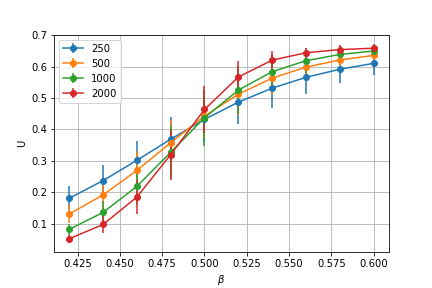
\includegraphics[width=0.7\textwidth]{images/Cumulant_beta0.4_0.6_no_title.png} 
	\caption{Graph of cumulants for conformations with lengths 250, 500, 1000, 2000, which were selected using radius of gyration. Here $\beta = \frac{1}{T}$ - inverse temperature, U - cumulant value.}
	\label{fig:cumulant}
\end{figure}

First approach was to use the radius of gyration as a parameter for differentiation: low radius - globule, high - coil. But as we can see on fig.\ref{fig:radius}, there are many conformations with similar radius of gyration (about 0.6) which have completely different magnetization values: from 0.2 to 1.0. Therefor this method requires us to mark many conformations that are possibly globular as coils, so we can not use it.
Although experiments with differentiation by radius of gyration show that it is possible to separate a set of globular conformations which have a magnetic transition, results are shown on fig. \ref{fig:cumulant}.

\begin{figure}
	\centering
	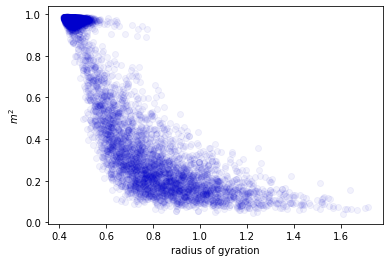
\includegraphics[width=0.6\textwidth]{images/mag2_to_R_L1000.png} 
	\caption{Graph of magnetization and radius of gyration for conformations of length 1000}
	\label{fig:radius}
\end{figure}

\begin{figure}
	\centering
	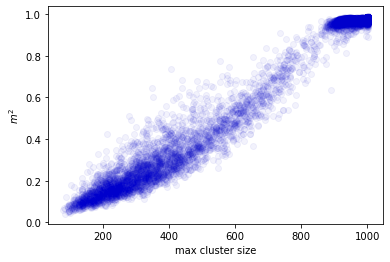
\includegraphics[width=0.6\textwidth]{images/mag_from_cluster_size.png} 
	\caption{Graph of magnetization and size of biggest cluster for conformations of length 1000}
	\label{fig:cluster_mag}
\end{figure}

Currently, the most promising way of differentiation is to find the biggest cluster(set of connected vertexes with 3 or more neighbors) in conformation, if its relative size to the size of the whole conformation is big enough, then it is a globular conformation. As we can see on fig. \ref{fig:cluster_mag} the difference in magnetization among conformations with the same cluster size is low, therefor differentiation can be much clearer.
	

\section*{Conclusion}
So far we can not confirm that the magnetic transition exists in globular conformations, but we see strong evidences of that. We have found correlation between the size of clusters in conformation, and it's magnetization.  We will continue experiments with different methods of differentiation of conformations, to determine the transition point.



\begin{thebibliography}{7}
	\bibitem{Ising_model}
		Ernst Ising, Contribution to the Theory of Ferromagnetism, 1925
	\bibitem{wolff_algo}
		U. Wolff, Collective Monte Carlo Updating for Spin Systems. Physical Review Letters. 62 (4): 361–364, 1989
	\bibitem{supercomputer}
		Kostenetskiy P.S., Chulkevich R.A., Kozyrev V.I. HPC Resources of the Higher School of Economics // Journal of Physics: Conference Series. 2021. Vol. 1740, No. 1. P. 012050. DOI: https://doi.org/10.1088/1742-6596/1740/1/012050
	\bibitem{github}
		Github repository link https://github.com/MoskalenkoRomanBorisovich/Ising-on-random-conformation
	\bibitem{Binder_cumulant}
		K. Binder, Finite size scaling analysis of ising model block distribution functions. Zeitschrift für Physik B: Condensed Matter. 43 (2): 119–140, 1981

\end{thebibliography}

\end{document}